\documentclass[11pt,a4paper]{report}
\usepackage[portuges]{babel}
\usepackage[utf8]{inputenc} 
\usepackage{graphicx} 
\usepackage{url} 
\usepackage{enumerate} 
\usepackage{color} 
\usepackage{textcomp}
\usepackage{indentfirst}
\usepackage{array} 
\usepackage{parskip}
\usepackage[export]{adjustbox}
\usepackage{xpatch}
\newlength{\chaptertopskip}
\setlength{\chaptertopskip}{10pt}

\usepackage{a4wide}
\usepackage{float}
\usepackage{minted}
\usepackage{multicol}
\usepackage{appendix}
\setlength{\parskip}{1em}
\usepackage{verbatim}

\usepackage[demo]{graphicx}
\usepackage{caption}
\usepackage{subcaption}


\usepackage[pdftex]{hyperref} % transformar as referências internas do seu documento em hiper-ligações.

\definecolor{saddlebrown}{rgb}{0.55, 0.27, 0.07} % para definir uma nova cor, neste caso 'saddlebrown'

\usepackage{listings}  % para utilizar blocos de texto verbatim no estilo 'listings'
%paramerização mais vulgar dos blocos LISTING - GENERAL
\lstset{
	basicstyle=\small, %o tamanho das fontes que são usadas para o código
	numbers=left, % onde colocar a numeração da linha
	numberstyle=\tiny, %o tamanho das fontes que são usadas para a numeração da linha
	numbersep=5pt, %distancia entre a numeração da linha e o codigo
	breaklines=true, %define quebra automática de linha
    frame=tB,  % caixa a volta do codigo
	mathescape=true, %habilita o modo matemático
	escapeinside={(*@}{@*)} % se escrever isto  aceita tudo o que esta dentro das marcas e nao altera
}

\usepackage{xspace} % deteta se a seguir a palavra tem uma palavra ou um sinal de pontuaçao se tiver uma palavra da espaço, se for um sinal de pontuaçao nao da espaço

\parindent=20pt %espaço a deixar para fazer a  indentação da primeira linha após um parágrafo
\parskip=10pt % espaço entre o parágrafo e o texto anterior

\setlength{\oddsidemargin}{-1cm} %espaço entre o texto e a margem
\setlength{\textwidth}{18cm} %Comprimento do texto na pagina
\setlength{\headsep}{0cm} %espaço entre o texto e o cabeçalho
\setlength{\textheight}{23cm} %altura do texto na pagina
\renewcommand{\baselinestretch}{1.5cm}


\begin{document}
\begin{figure}
    
\includegraphics[scale=0.3]{logoum.png}
\end{figure}
\title{\textbf{Primitivas Gráficas}\\
       \textbf{Unidade Curricular de Computação Gráfica}\\ Licenciatura em Ciências da Computação\\Universidade do Minho
       } %Titulo do documento
\author{Bruno Jardim\\ (A91680) \and Inês Presa\\ (A90355)
         \and Tiago Carriço\\ (A91695) \and Tiago Leite\\ (A91693)
       } %autores do documento
\date{\today} %data
\maketitle
\begingroup
\renewcommand*\contentsname{Índice}
\let\clearpage\relax
\tableofcontents


\endgroup
\newpage

\chapter{Contextualização}    
No âmbito da unidade curricular de Computação Gráfica da Licenciatura em Ciências da Computação foi proposta o desenvolvimento em \textit{Opengl} de um motor gráfico genérico que terá como função a criação de um sistema solar. Desenvolvimento esse que deve ser composto por quatro etapas. 

\section{Enunciado}
Nesta primeira etapa foi proposta a criação de duas aplicações:

\begin{itemize}
    \item \textbf{Gerador}
        \begin{description}
        \item Funcionalidade: Gerar ficheiros com os pontos no espaço necessários para desenhar primitivas gráficas, como por exemplo, planos, cubos, esferas e cones.
        \end{description}

    \item \textbf{Motor Gráfico}
    \begin{description}
    \item Funcionalidade: Interpretar um ficheiro XML com a configuração da câmara e os ficheiros com os pontos previamente gerados, e desenhar as primitivas.
    \end{description}
\end{itemize}


\chapter{Apresentação das soluções}
\section{Gerador}
O gerador permite, através de um conjunto de parâmetros, gerar diversos tipos de primitivas gráficas, escrevendo as coordenadas dos pontos que compõem a primitiva pretendida num ficheiro com extensão \textit{.3d} para mais tarde ser carregado e utilizado pelo motor gráfico.

\subsection{Plano}
\vspace{0.5cm}
Para gerar o plano iterou-se no comprimento e largura do mesmo através de dois ciclos \textit{for}, partindo do canto cujas coordenadas \textit{x} e \textit{z} são negativas, percorrendo cada linha e desenhando simultaneamente os dois triângulos que constituem cada secção do plano. 
\vspace{1cm}
\begin{figure}[H]
\centering
\begin{subfigure}{0.5\textwidth}
  \centering
  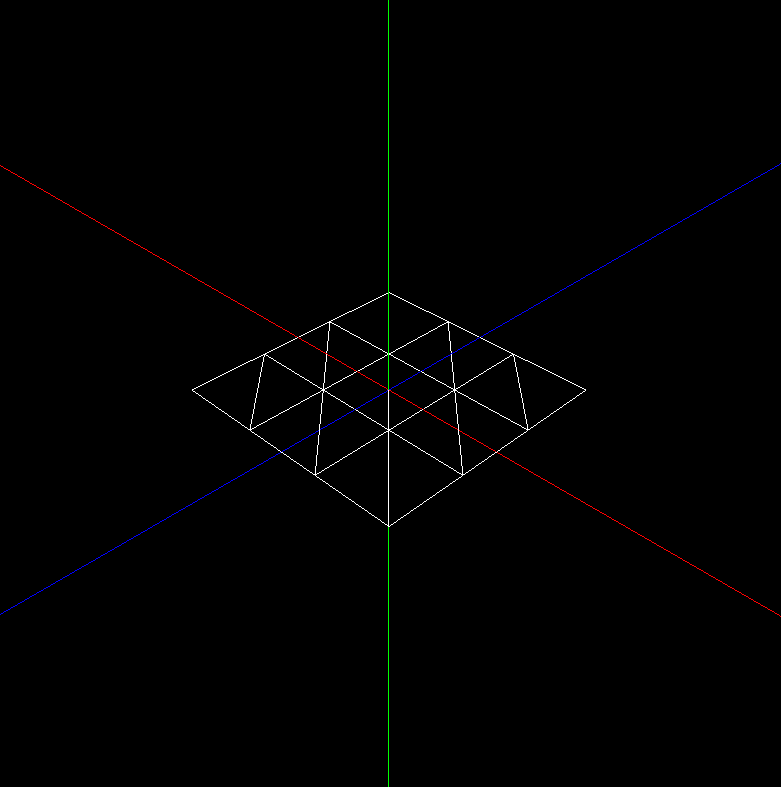
\includegraphics[width = 8cm,height = 8cm]{plano1.png}
  \caption{\texttt{./generator plane 1 3 plane.3d}}
  \label{fig:plano1}
\end{subfigure}%
\begin{subfigure}{0.5\textwidth}
  \centering
  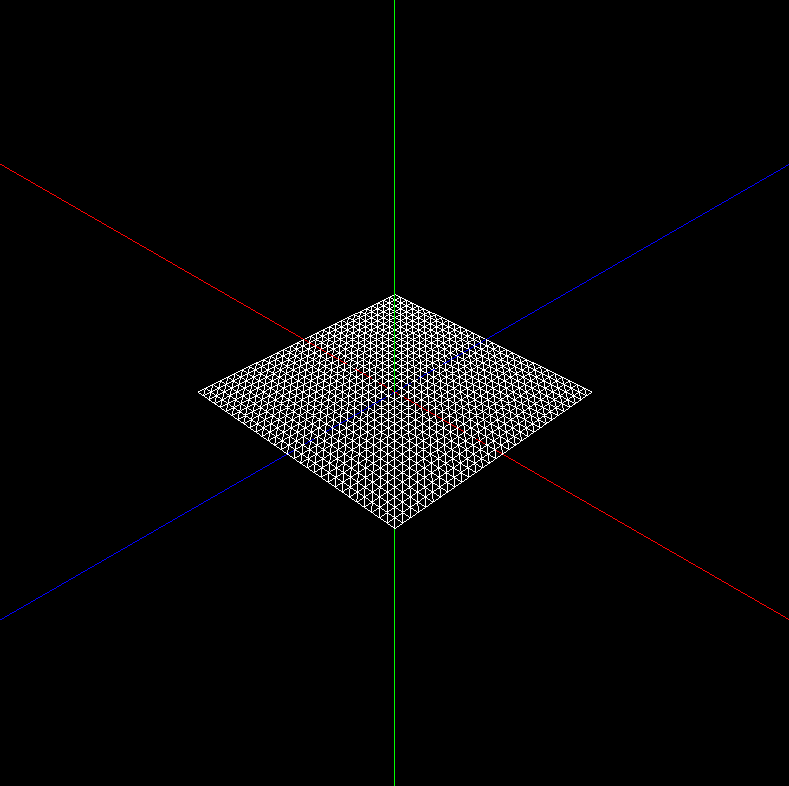
\includegraphics[width = 8cm,height = 8cm]{plano2.png}
  \caption{\texttt{./generator plane 1 30 plane.3d}}
  \label{fig:plano2}
\end{subfigure}
\caption{Exemplos de planos}
\label{fig:plano}
\end{figure}


\newpage
\subsection{Caixa}
\vspace{0.5cm}
Com a primitiva do plano feita, facilmente se chegou à caixa, uma vez que esta é obtida através de 6 planos paralelos, dois a dois e a cada um dos planos coordenados. Sendo que se deu atenção à sua orientação para que sejam visíveis de fora da caixa.
\vspace{1cm}
\begin{figure}[H]
\centering
\begin{subfigure}{0.5\textwidth}
  \centering
  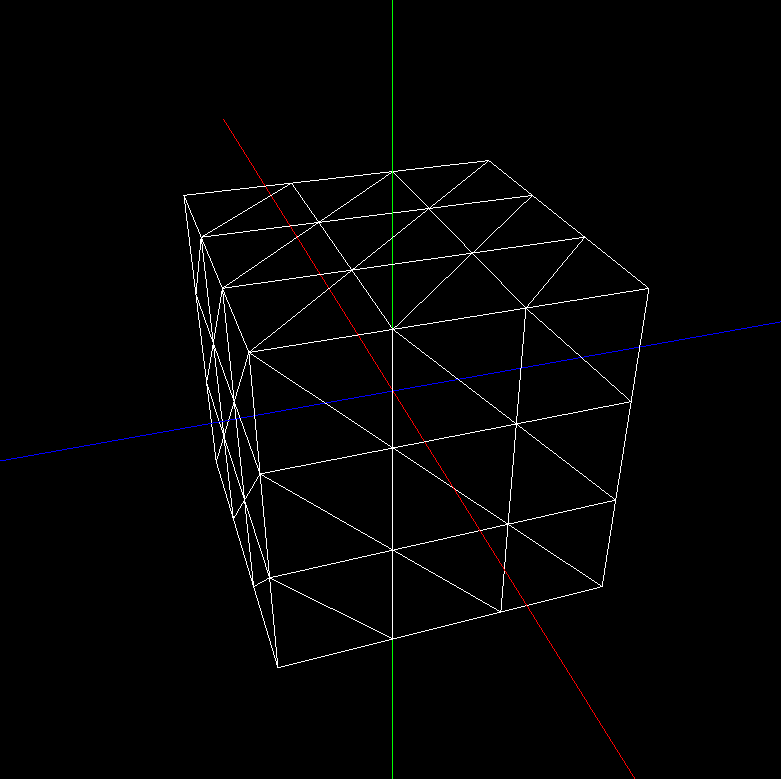
\includegraphics[width = 8cm,height = 8cm]{caixa1.png}
  \caption{\texttt{./generator box 2 3 box.3d}}
  \label{fig:caixa1}
\end{subfigure}%
\begin{subfigure}{0.5\textwidth}
  \centering
  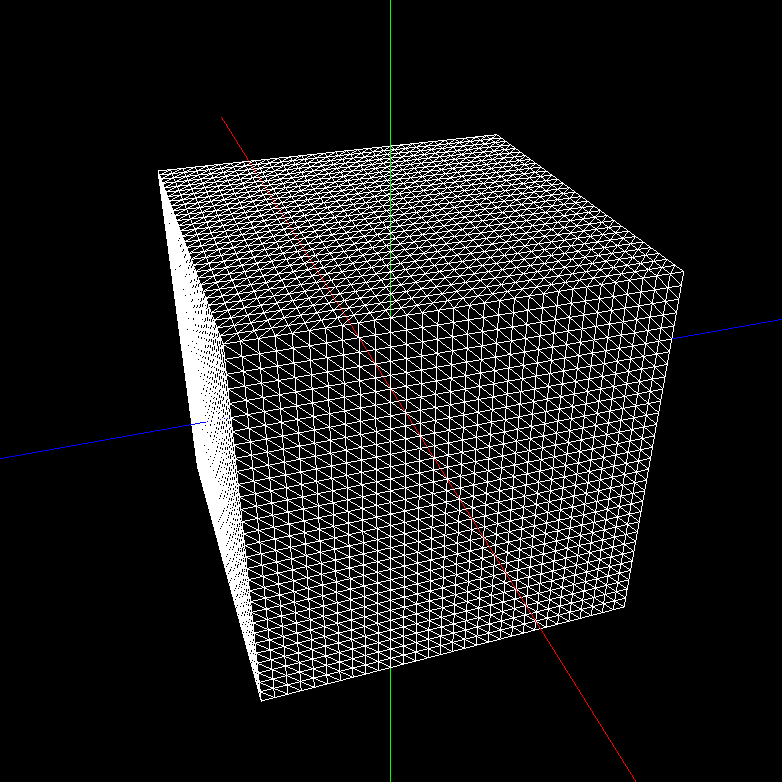
\includegraphics[width = 8cm,height = 8cm]{caixa2.png}
  \caption{\texttt{./generator box 2 30 box.3d}}
  \label{fig:caixa2}
\end{subfigure}
\caption{Exemplos de caixas}
\label{fig:caixa}
\end{figure}
\newpage

\subsection{Esfera}
\vspace{0.5cm}
Começando no pólo superior e iterando por cada \textit{slice} da esfera, construiu-se o sólido, utilizando coordenadas polares para que fosse possível descrever com precisão as coordenadas de cada ponto da esfera, tornando assim a representação o mais fiel possível.
\vspace{1cm}
\begin{figure}[H]
\centering
\begin{subfigure}{0.5\textwidth}
  \centering
  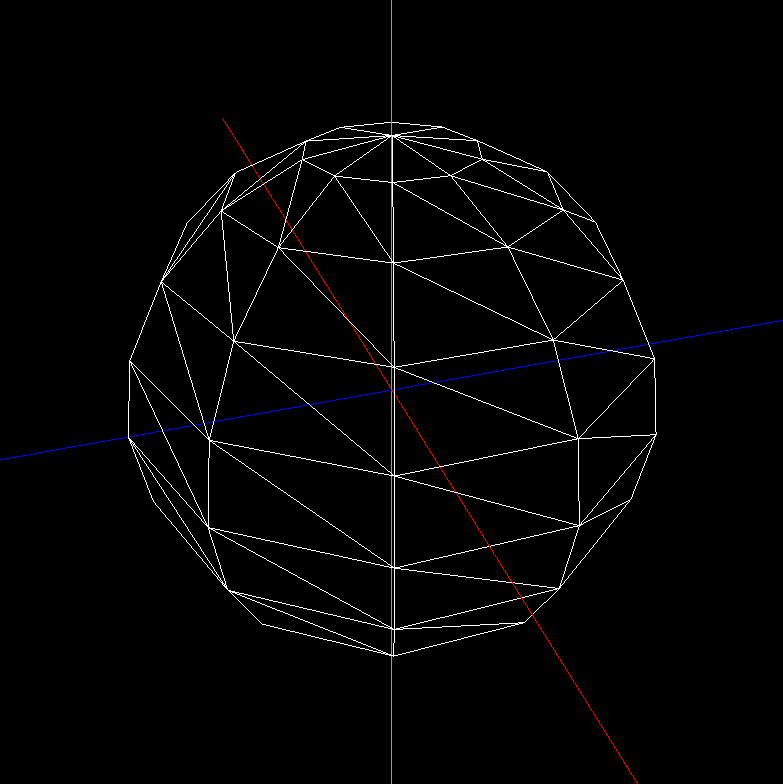
\includegraphics[width = 8cm,height = 8cm]{esfera1.png}
  \caption{\texttt{./generator sphere 1 10 10 sphere.3d}}
  \label{fig:esfera1}
\end{subfigure}%
\begin{subfigure}{0.5\textwidth}
  \centering
  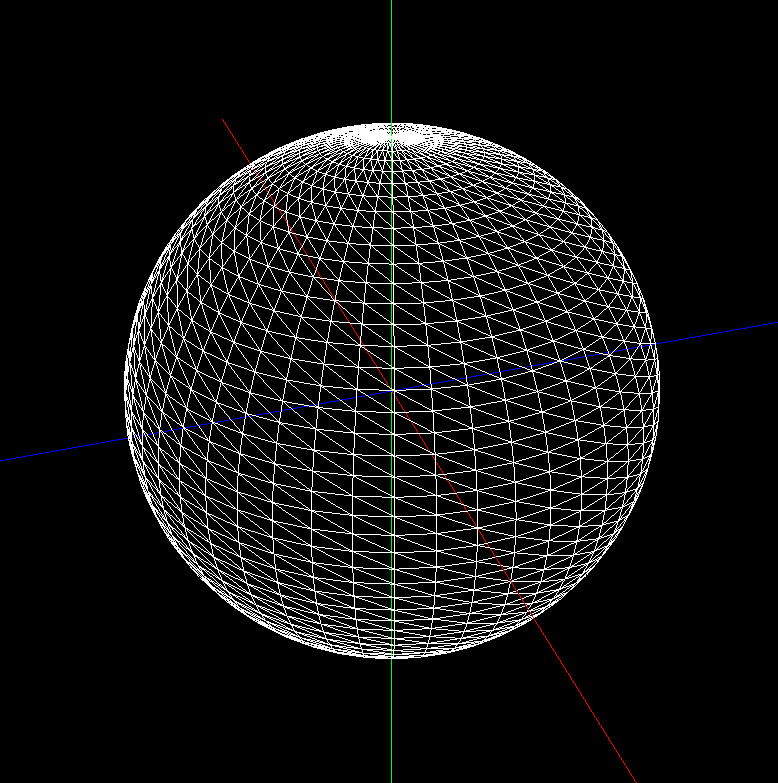
\includegraphics[width = 8cm,height = 8cm]{esfera2.png}
  \caption{\texttt{./generator sphere 1 50 50 sphere.3d}}
  \label{fig:esfera2}
\end{subfigure}
\caption{Exemplos de esferas}
\label{fig:esfera}
\end{figure}
\newpage
\subsection{Cone}
\vspace{0.5cm}
Tendo como ponto de partida a origem do referencial criou-se um circulo sobre o plano \textit{$y = 0$}, este será a base do cone. Com isto foi desenhada, \textit{stack} por \textit{stack}, a face do cone, mais uma vez, utilizando coordenadas polares e o teorema de Tales para descobrir o valor do raio em cada \textit{stack}.
\vspace{1cm}
\begin{figure}[H]
\centering
\begin{subfigure}{0.5\textwidth}
  \centering
  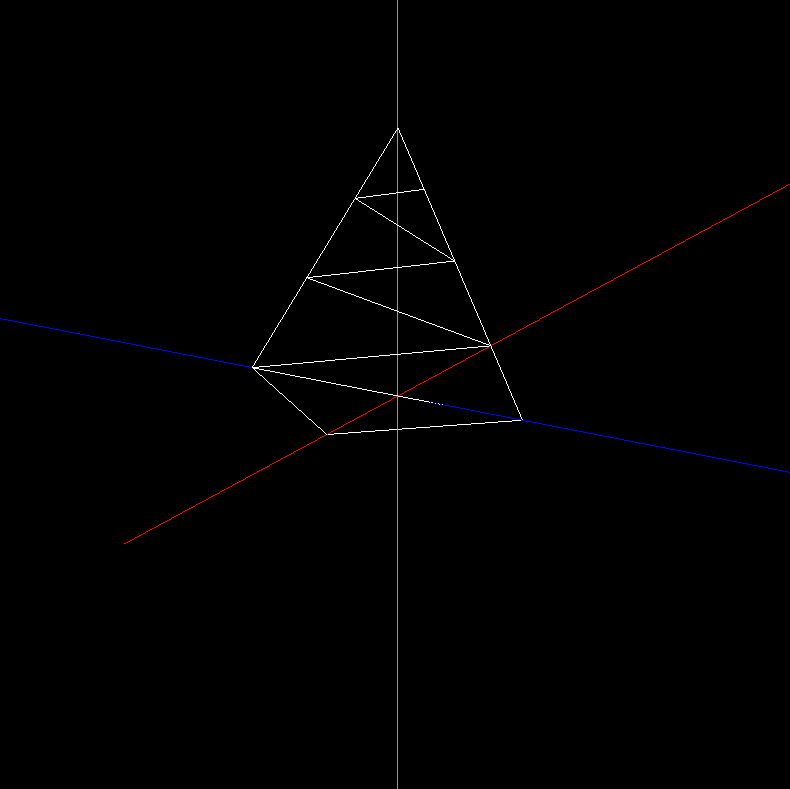
\includegraphics[width = 8cm,height = 8cm]{cone1.png}
  \caption{\texttt{./generator cone 1 2 4 3 cone.3d}}
  \label{fig:cone1}
\end{subfigure}%
\begin{subfigure}{0.5\textwidth}
  \centering
  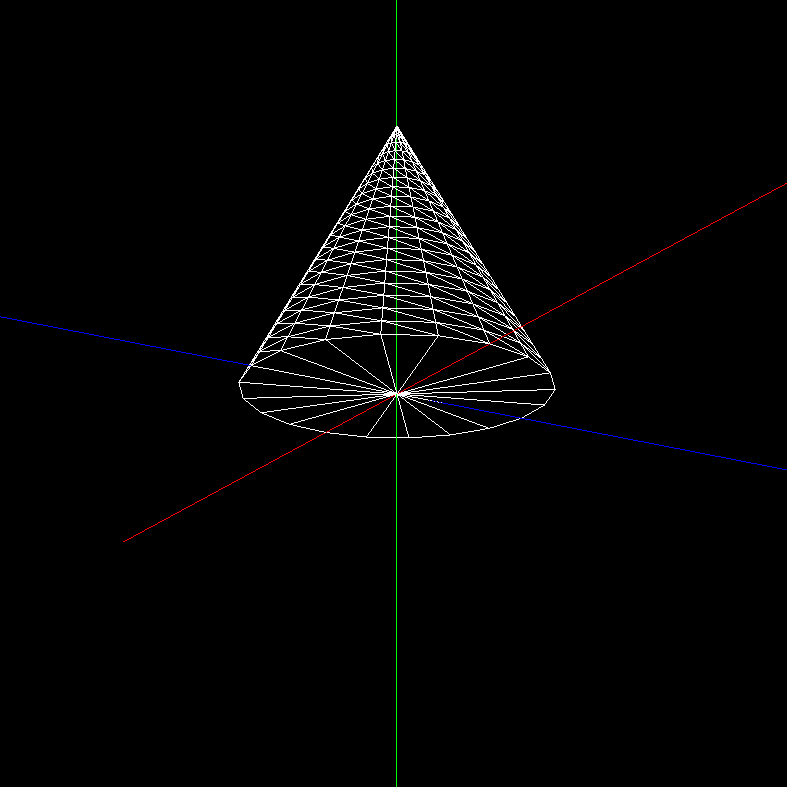
\includegraphics[width = 8cm,height = 8cm]{cone2.png}
  \caption{\texttt{./generator cone 1 2 20 20 cone.3d}}
  \label{fig:cone2}
\end{subfigure}
\caption{Exemplos de cones}
\label{fig:cone}
\end{figure}
\newpage
\subsection{Cilindro}
\vspace{0.5cm}
Utilizando o cilindro desenvolvido nas aulas, foi introduzido um novo parâmetro, o numero de \textit{stacks}, pois assim consegue-se um nível de detalhe superior no cilindro.
Com a estratégia usada para construir o cone, fez-se uma alteração para que o raio do cilindro não diminuísse com o aumento da altura, em oposição ao que acontece no caso do cone.
\vspace{1cm}
\begin{figure}[H]
\centering
\begin{subfigure}{0.5\textwidth}
  \centering
  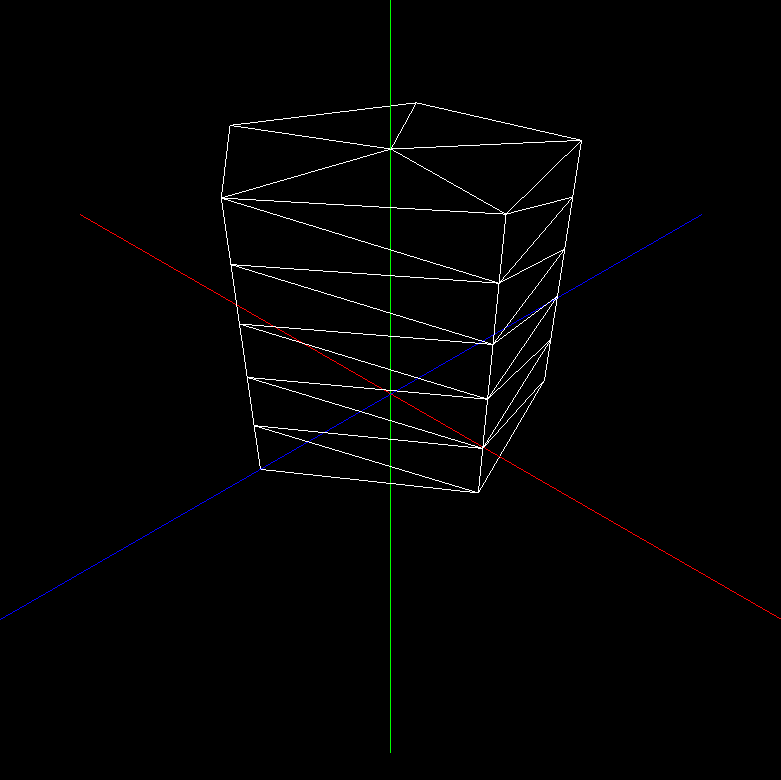
\includegraphics[width = 8cm,height = 8cm]{cilindro1.png}
  \caption{\texttt{./generator cylinder 2 3 5 5 cylinder.3d}}
  \label{fig:cylinder1}
\end{subfigure}%
\begin{subfigure}{0.5\textwidth}
  \centering
  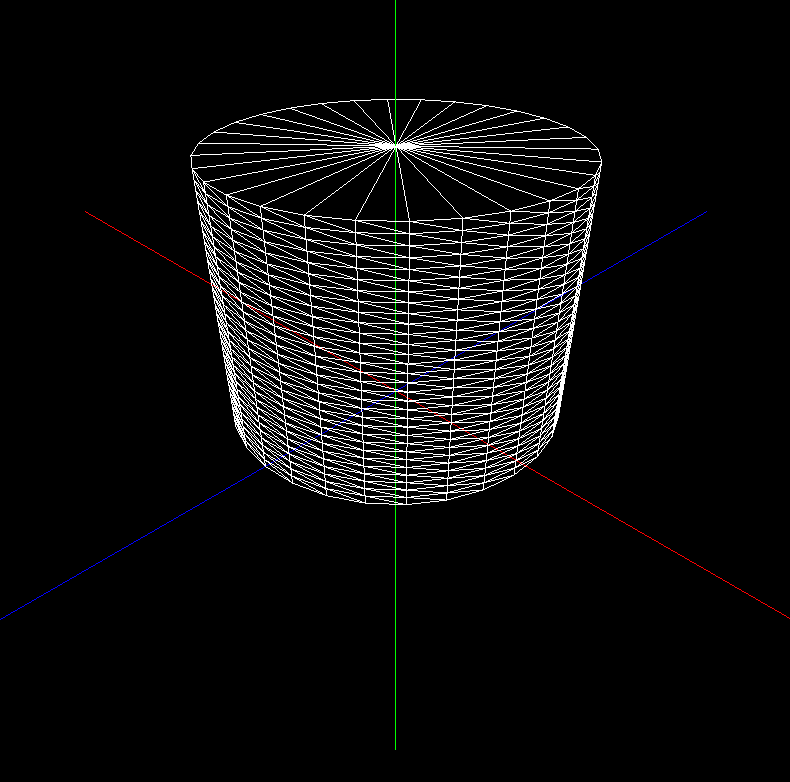
\includegraphics[width = 8cm,height = 8cm]{cilindro2.png}
  \caption{\texttt{./generator cylinder 2 3 30 30 cylinder.3d}}
  \label{fig:cylinder2}
\end{subfigure}
\caption{Exemplos de cilindros}
\label{fig:cylinder}
\end{figure}
\newpage
\subsection{Torus}
\vspace{0.5cm}
Através das fórmulas disponibilizadas \href{https://en.wikipedia.org/wiki/Torus#Geometry}{\textbf{aqui}}, conseguiu-se gerar uma representação de um \textit{torus}, algo que futuramente vai permitir desenhar os vários anéis dos planetas do sistema solar.
\vspace{1cm}
\begin{figure}[H]
\centering
\begin{subfigure}{0.5\textwidth}
  \centering
  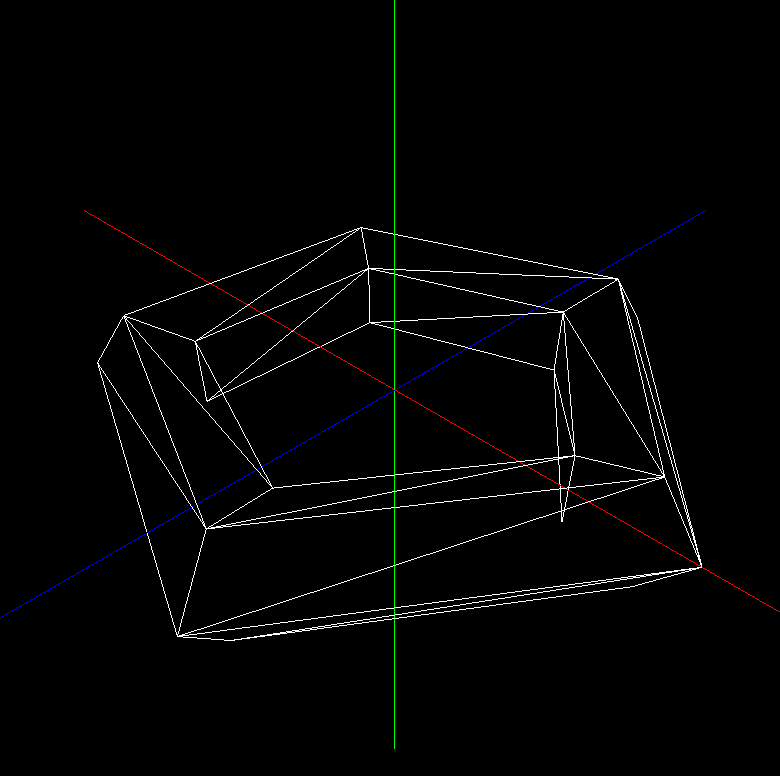
\includegraphics[width = 8cm,height = 8cm]{torus1.png}
  \caption{\texttt{./generator torus 5 3 5 5 torus.3d}}
  \label{fig:torus1}
\end{subfigure}%
\begin{subfigure}{0.5\textwidth}
  \centering
  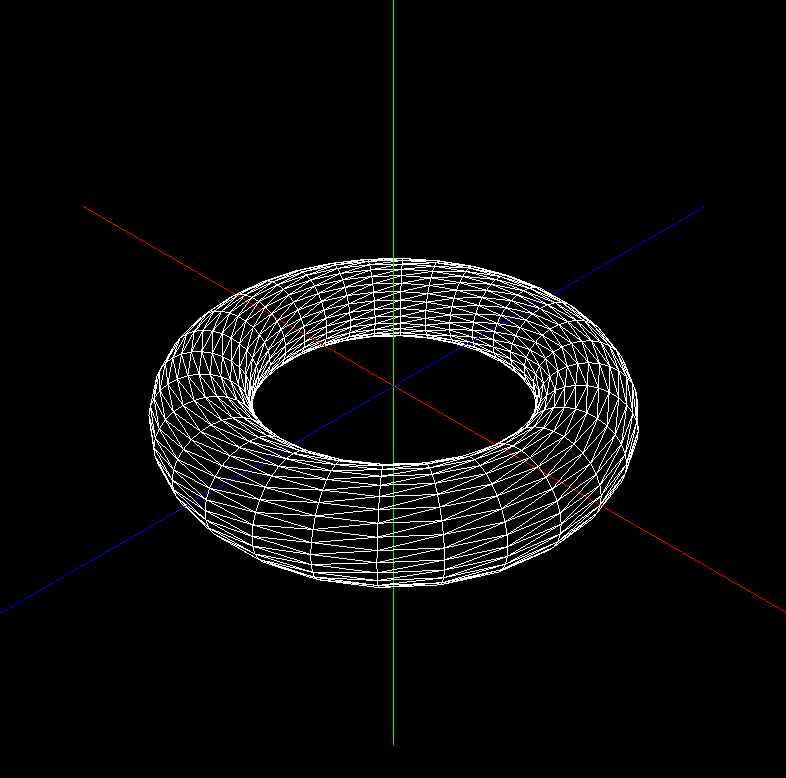
\includegraphics[width = 8cm,height = 8cm]{torus2.png}
  \caption{\texttt{./generator torus 5 3 30 30 torus.3d}}
  \label{fig:torus2}
\end{subfigure}
\caption{Exemplo de torus}
\label{fig:torus}
\end{figure}
\newpage
\section{Motor Gráfico}
O motor gráfico interpreta um ficheiro XML e com a informação nele contido irá gerar uma cena. Para que o motor tivesse esta funcionalidade, tomou-se vantagem do \textit{parser} \href{http://www.grinninglizard.com/tinyxml/}{\textbf{tinyXML}}.
Após ser executado o \textit{parser} extrai a seguinte informação do ficheiro:
\begin{itemize}
    \item Câmara
    \begin{itemize}
        \item Posição da câmara (\textit{position})
        \item Ponto para onde a câmara está a olhar (\textit{lookAt})
        \item Inclinação da câmara (\textit{up})
        \item \textit{View Frustum} 
    \end{itemize}
    \item Modelos
    \begin{itemize}
        \item Nome dos ficheiros \textit{.3d} a carregar
        
    \end{itemize}
    
    
    
\end{itemize}

Após carregar os ficheiros \textit{.3d} os pontos neles contidos são armazenados num vetor de vetores de \textit{Point}, uma estrutura de dados previamente definida, que representa um ponto no espaço. Cada vetor armazena os pontos constituintes de uma primitiva gráfica, permitindo assim carregar múltiplas primitivas na mesma cena.

\newline 
Mais ainda, o  motor gráfico tem implementado uma câmara em modo \textit{explorer} que  permite rodar em torno da cena através das \textit{arrowkeys} e com as teclas \textit{Page Up} e \textit{Page Down} possibilita aproximar e afastar, respetivamente, a câmara da origem do referencial.


\newpage
\chapter{Conclusão}
A principal dificuldade enfrentada durante esta fase do trabalho foi, inicialmente a adaptação às coordenadas polares, logo ambos o cone e a esfera tornaram-se um desafio. No entanto considera-se que foi ultrapassada agilmente.

A adaptação à linguagem foi também uma dificuldade, já que nenhum elemento do grupo tinha experiência prévia com a linguagem em questão, nomeadamente \texttt{\textbf{C++}}. 

Por último, a utilização do \href{http://www.grinninglizard.com/tinyxml/}{\textbf{parser de XML}} de terceiros também condicionou o nosso progresso uma vez que o grupo não estava familiarizado com a ferramenta.

Concluindo, apesar das dificuldades enfrentadas, os objetivos foram atingidos prontamente, no que o grupo considera ser um balanço muito positivo.
\end{document}
